\documentclass[12pt, a4paper]{article}

\usepackage[hmargin=2.5cm, vmargin=2cm]{geometry}
\usepackage{amsthm, amssymb, mathtools, yhmath, graphicx}
\usepackage{fontspec, type1cm, titlesec, titling, fancyhdr, tabularx}
\usepackage{caption}
\usepackage{color}
\usepackage{hhline}
\usepackage{unicode-math}
\usepackage{nicefrac}
\usepackage[abbreviations]{siunitx}
\usepackage{comment}
\usepackage{float}
\usepackage{subcaption}

\usepackage[CheckSingle, CJKmath]{xeCJK}
\usepackage{CJKulem}
\usepackage{enumitem}
\usepackage[usenames, dvipsnames]{xcolor}
\usepackage{colortbl}
\usepackage{circuitikz}
%\setCJKmainfont[BoldFont=cwTex Q Hei]{cwTex Q Ming}
%\setCJKsansfont[BoldFont=cwTex Q Hei]{cwTex Q Ming}
%\setCJKmonofont[BoldFont=cwTex Q Hei]{cwTex Q Ming}
\setCJKmainfont[BoldFont=cwTeX Q Hei]{cwTeX Q Ming}

\def\normalsize{\fontsize{12}{18}\selectfont}
\def\large{\fontsize{14}{21}\selectfont}
\def\Large{\fontsize{16}{24}\selectfont}
\def\LARGE{\fontsize{18}{27}\selectfont}
\def\Huge{\fontsize{20}{30}\selectfont}

\titleformat{\section}{\bf\Large}{\arabic{section}}{24pt}{}
\titleformat{\subsection}{\large}{\arabic{subsection}.}{12pt}{}
\titlespacing*{\subsection}{0pt}{0pt}{1.5ex}

\parindent=24pt

\DeclarePairedDelimiter{\abs}{\lvert}{\rvert}
\DeclarePairedDelimiter{\norm}{\lVert}{\rVert}
\DeclarePairedDelimiter{\inpd}{\langle}{\rangle}
\DeclarePairedDelimiter{\ceil}{\lceil}{\rceil}
\DeclarePairedDelimiter{\floor}{\lfloor}{\rfloor}

\newcommand{\unit}[1]{\:(\text{#1})}
\newcommand{\img}{\mathsf{i}}
\newcommand{\ex}{\mathsf{e}}
\newcommand{\dD}{\mathrm{d}}
\newcommand{\dI}{\,\mathrm{d}}
\DeclareSIUnit \uF {\micro \farad}
\DeclareSIUnit \mH {\milli \henry}

\title{ \bf {\huge 電子電路實驗10:方波的諧波分析}\\ 實驗預報}
\author{B02901178 江誠敏}
%\date{2014/09/21}

\begin{document}

\maketitle

\section{實驗目的}
我們從傅立葉級數理論(Fourier series Theory)可知,方波是由一連串之弦波(sinusoidal wave)
所合成的,本實驗將利用前一個實驗所介紹的帶通濾波器(band-pass filter)把潛藏於方波之中
的弦波成分找出來。


\section{實驗步驟}
\begin{enumerate}[itemsep=0pt]
\item 以 LCR 計量測各個電容與電感的值,並用數位電表量測各個固定電阻的值。
\item 將電路連接如圖 10.1(c)所示,其中 $R_1 = R_3 = \SI{510}{\ohm} $, $R_2 = \SI{100}{\ohm}$, $R_6 = \SI{10}{\kohm} $, $C_4 = \SI{0.01}{\uF} $,
$C_6 = \SI{0.01}{\uF} $,OP 電源為±15V,+K 的放大電路直接短路至 $v_o$ 即可。用可變電阻將 $R_5$ 值調
整至10kΩ 附近(不用太準)。
\item 令 $v_i$為高低電位差 1V (1V 是信號產生器已接上電路的值),頻率為 1kHz 的方波。微調可
變電阻 $R_5$,使得 $v_o$ 近似於一個頻率與方波相同,且振幅為最大的弦波。將此時的 $v_i$以及
$v_o$ 記錄於方格紙上,並以數位電表量測此時的 $R_5$ 之電阻值。
\item 用可變電阻將 $R_5$ 值調整至1.1kΩ 附近(不用太準),將電源與 $v_i$接上之後可見 $v_o$ 為一個頻
率約為方波的 3 倍的類似弦波。微調可變電阻 $R_5$,使得 $v_o$ 的頻率維持在這附近,且振幅
為最大。將此時的 $v_i$以及 $v_o$ 記錄於方格紙上,並以數位電表量測此時的 $R_5$ 之電阻值。
\item 用可變電阻將 $R_5$ 值調整至400Ω 附近(不用太準),將電源與 $v_i$ 接上之後可見 $v_o$ 為一個頻
率約為方波的 5 倍的類似弦波。微調可變電阻 $R_5$,使得 $v_o$ 的頻率維持在這附近,且振幅
為最大。將此時的 $v_i$以及 $v_o$ 記錄於方格紙上,並以數位電表量測此時的 $R_5$ 之電阻值。
\item 用可變電阻將 $R_5$ 值調整至200Ω 附近(不用太準),將電源與 $v_i$ 接上之後可見 $v_o$ 為一個頻
率約為方波的 7 倍的類似弦波。微調可變電阻 $R_5$,使得 $v_o$ 的頻率維持在這附近,且振幅
為最大。將此時的 $v_i$以及 $v_o$ 記錄於方格紙上,並以數位電表量測此時的 $R_5$ 之電阻值。
\item 將可變電阻 $R_5$ 調回步驟 3 量得的值,分別調整方波頻率為 333Hz、200Hz、142.9Hz,觀
察並將此時的 $v_i$以及 $v_o$ 記錄於方格紙上。
\end{enumerate}


\section{預報問題}

\begin{enumerate}[itemsep=20pt, topsep=10pt]
  \item {\large\bf 請推導 $\text{Duty Cycle} =50\%$ 的方波的傅立葉級數,以驗證實驗原理中的關係式。} \\[10pt]
    假設方波的函數為
    \[
      f(t) = 
      \begin{dcases}
        V, & \text{if } t \in [2n\pi, (2n+1)\pi) \\
        -V, & \text{otherwise}
      \end{dcases}
    \]
    則
    \begin{align*}
      \mathfrak{F}(k) &= \frac{1}{2\pi} \int_{-\pi}^{\pi} f(t) e^{- \img k t} \dI t  = \frac{1}{2\pi} \int_{-\pi}^{0} f(t) e^{- \img k t} \dI t +  \frac{1}{2\pi} \int_{0}^{\pi} f(t) e^{- \img k t} \dI t  \\
                      &= V \frac{2 - e^{\img k t} + e^{- \img k t}}{\img k}  \\
      & = \frac{2V}{\pi} \frac{ [[ k = 2n + 1 ]] }{\img k}  
    \end{align*}
    所以
    \[
      f = \sum \mathfrak{F}(k) e^{\img k t} = \sum_{-\infty}^{\infty} \frac{2V}{\img (2n+1) \pi} e^{i(2n+1)t} = \frac{4V}{\pi} \sum_{0}^{\infty} \frac{\sin ((2n+1) t)}{2n+1}
    \]
    因此
    \begin{align*}
      a_1:a_2:a_3 \cdots &= \frac{1}{1} : \frac{1}{3} : \frac{1}{5}   \cdots \\
      \omega_1:\omega_2:\omega_3 \cdots &= 1:3:5 \cdots
    \end{align*}
  \item {\large\bf 欲將帶通濾波器之中心頻率調整為 1kHz,$R_5$應調整到多少?等效電感的值為多少?請推導之。}  \\[10pt]
    在實驗9已經計算過這個電路的Transfer function為
    \[
      f(s) = \frac{sL}{s^2LRC + sL + R} = \frac{L}{sLRC + L + R/s} 
    \]
    跟據算幾不等式,可知
    \[
      \abs*{f(\img \omega)} = \frac{L}{\abs{\img \omega LRC - \img R/\omega+L}} \leq \frac{L}{L} = 1
    \]
    等式成立若且唯若
    \[
      \omega LRC = \frac{R}{\omega} \quad \Leftrightarrow \quad \omega = \frac{1}{\sqrt{LC}}
    \]
    代入$\omega = 2 \pi f, f = \SI{1}{\kHz} $可以得到$L_{eq} \approx \SI{0.253}{\henry}$ 
    在代入
    \[
      sL = Z_L = \frac{s C_4 R_1 R_3 R_5}{R_2} 
    \]
    得出$R_5 = \SI{9739}{\ohm} $
  \item {\large\bf 請用 PSpice 或其他電路模擬軟體,模擬圖 10.1(c) 的電路,其中各元件值與方波的參數請依照步驟2 ,$R_5$ 的值請用預報問題2中的結果$r_0$。利用暫態分析的功能分別繪出當$R_5 = r_0, r_0/9, r_0/25, r_0/49$時,$v_o$與$v_i$ 的關係。}  \\[10pt]
    \begin{figure}[H]
      \centering
      \begin{subfigure}[b]{0.45\textwidth}
        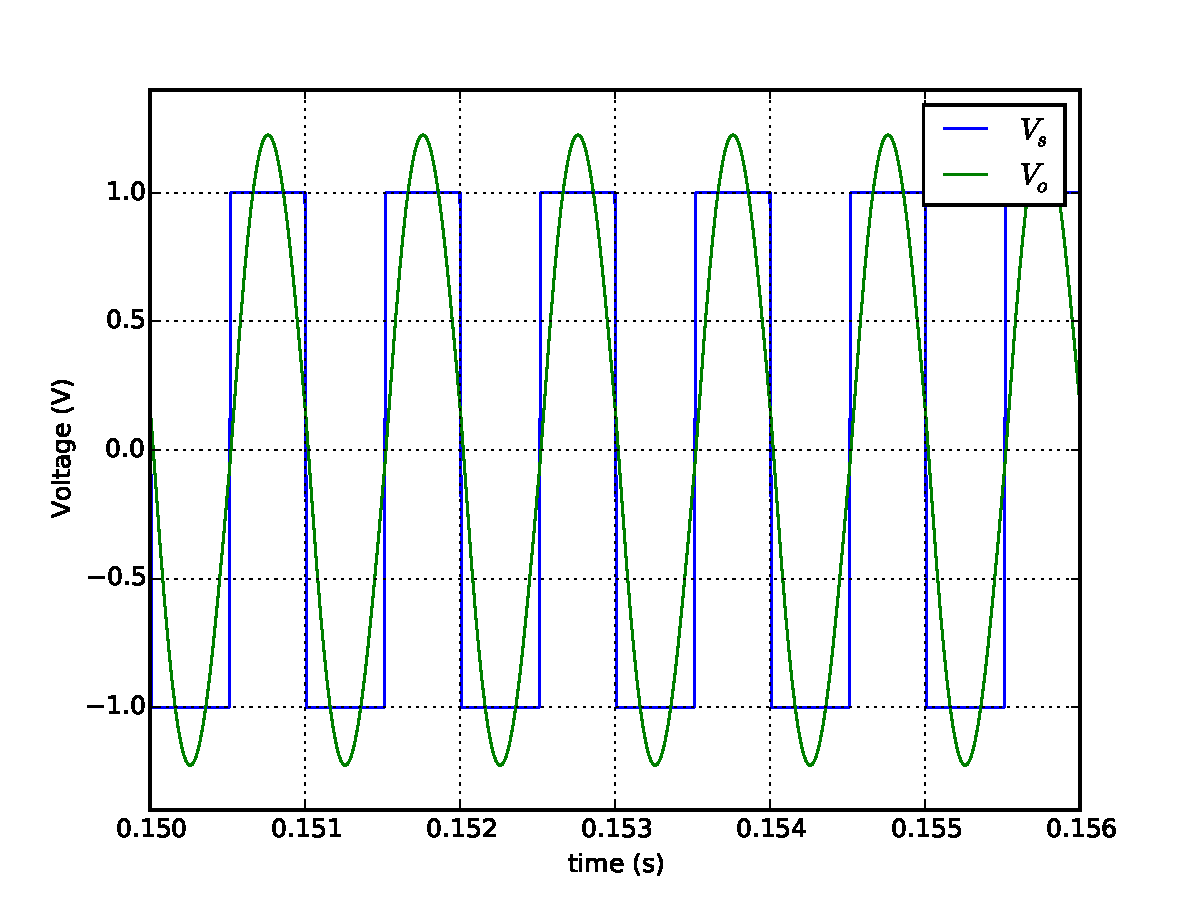
\includegraphics[width=1\textwidth]{circuit/p1.pdf}
        \caption{$R_5 = r_0 \approx \SI{9739}{\ohm} $}
      \end{subfigure}
      \begin{subfigure}[b]{0.45\textwidth}
        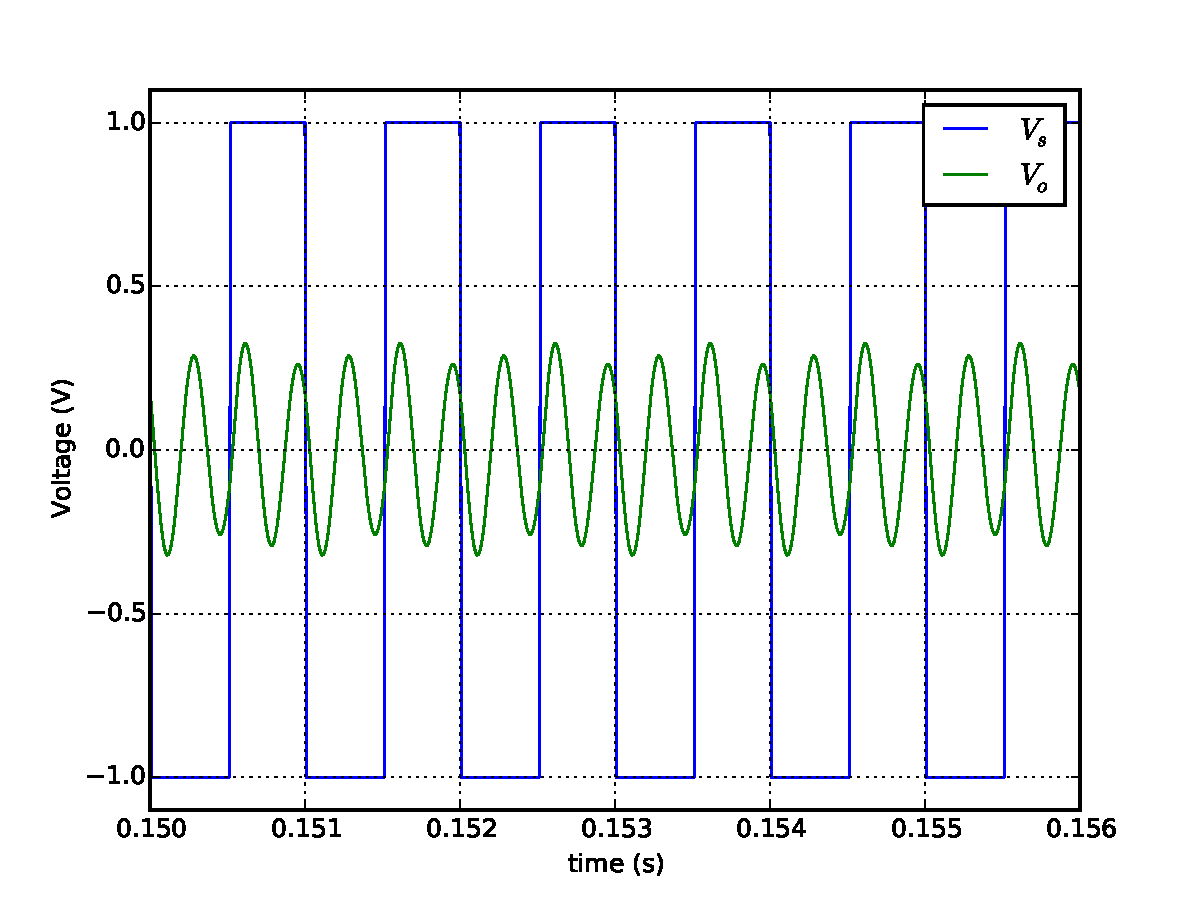
\includegraphics[width=1\textwidth]{circuit/p9.pdf}
        \caption{$R_5 = r_0 / 9 \approx \SI{1082}{\ohm} $}
      \end{subfigure}
      \begin{subfigure}[b]{0.45\textwidth}
        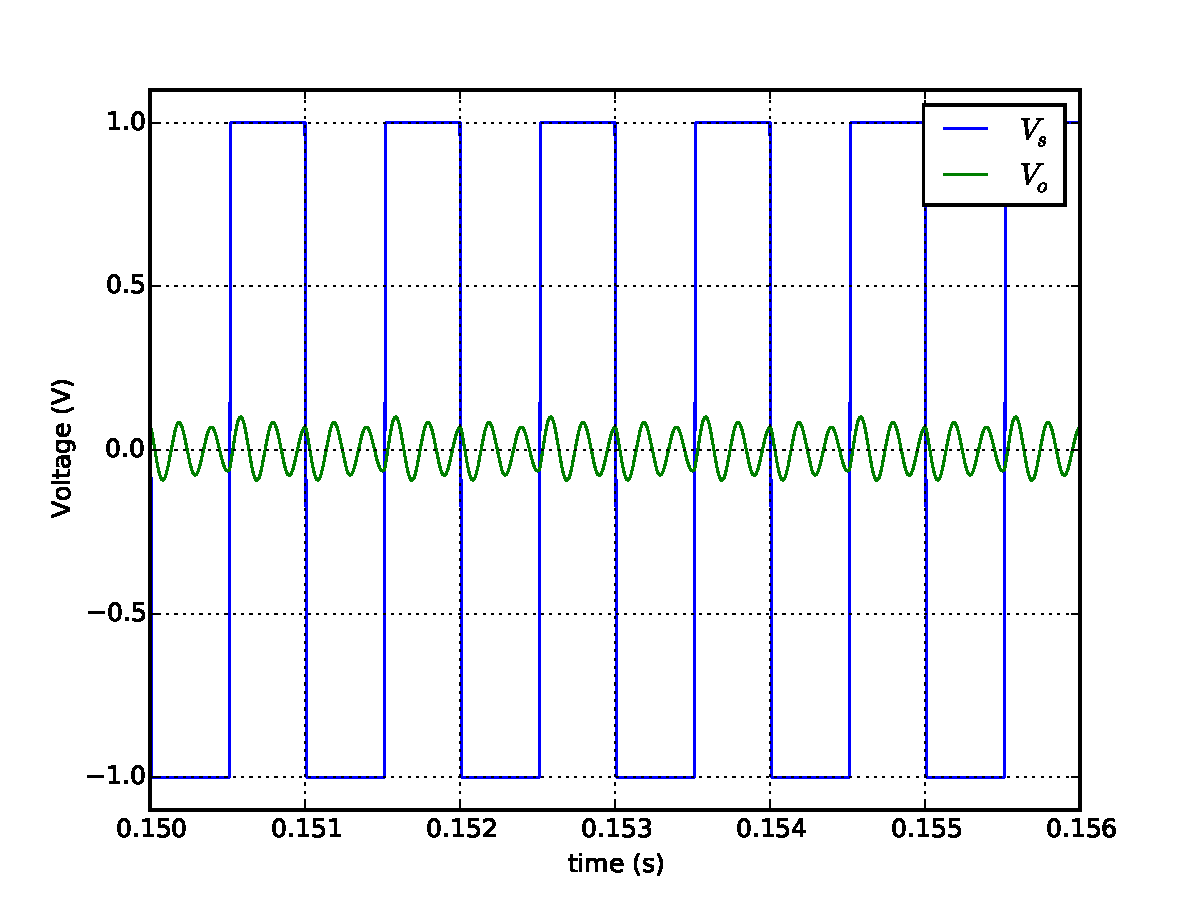
\includegraphics[width=1\textwidth]{circuit/p25.pdf}
        \caption{$R_5 = r_0 / 25 \approx \SI{389.6}{\ohm} $}
      \end{subfigure}
      \begin{subfigure}[b]{0.45\textwidth}
        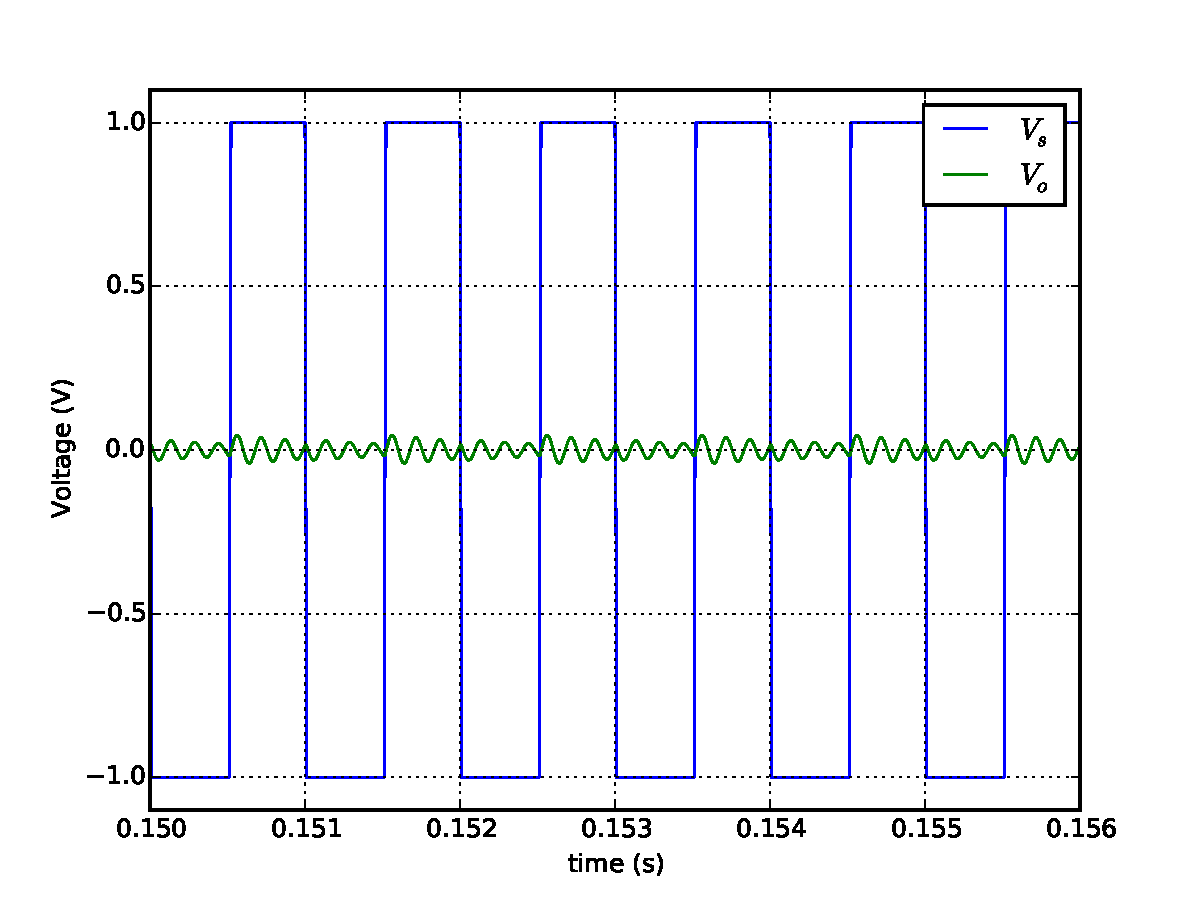
\includegraphics[width=1\textwidth]{circuit/p49.pdf}
        \caption{$R_5 = r_0 / 49 \approx \SI{198.8}{\ohm} $}
      \end{subfigure}
    \end{figure}

\end{enumerate}

\end{document}


